\documentclass[a4paper]{article}

%%% packages %%%%%%%%%%%%%%%%%%%%%%%%%%%%%%%%%%%%%%%%%%%%%%%%%%%%%%%%%%%%%%%%%
\usepackage{graphicx}
\usepackage{amsmath,amssymb}
\usepackage{alltt}
\usepackage{natbib} % please use \citep and \citet instead of \cite

\usepackage{hyperref}
\usepackage{xcolor}
\definecolor{dark-red}{rgb}{0.4,0.15,0.15}
\definecolor{dark-blue}{rgb}{0.15,0.15,0.8}
\definecolor{medium-blue}{rgb}{0,0,0.5}
\hypersetup{
	colorlinks, linkcolor={dark-red},
	citecolor={dark-blue}, urlcolor={medium-blue}
}

\graphicspath{{./figs/}}
\DeclareGraphicsExtensions{.pdf}

\setlength{\parindent}{0mm}

\usepackage{fancyhdr}

%%% %%%%%%%%%%%%%%%%%%%%%%%%%%%%%%%%%%%%%%%%%%%%%%%%%%%%%%%%%%%%%%%%%%%%%%%%%

\makeatletter
\newcommand{\seminar}{Seminar Cyber-Physical Systems (WS 2019/20)}
\title{\textbf{Prioritized Sweeping Neural DynaQ:\\ Boost Learning by Dreaming}}\let\Title\@title
\newcommand{\sTitle}{Prioritized Sweeping Neural DynaQ}
\newcommand{\AuthorName}{Alexander Osiik}
\author{\AuthorName\\
	\href{mailto:alexander.osiik@student.uni-luebeck.de}{alexander.osiik@student.uni-luebeck.de}\\
	\small \seminar\\
%	\small Service Robotics Group\\
	\small Institute of Computer Engineering, University of L\"ubeck\\
}\let\Author\@author
\makeatother

\pagestyle{fancy}
\renewcommand{\footrulewidth}{0.4pt}
\lfoot{\seminar}
\cfoot{}
\rfoot{\thepage}
\lhead{\AuthorName}
\rhead{\sTitle}

%%% %%%%%%%%%%%%%%%%%%%%%%%%%%%%%%%%%%%%%%%%%%%%%%%%%%%%%%%%%%%%%%%%%%%%%%%%%

\begin{document}
	\maketitle
	
	\begin{abstract}
		\noindent%
		Hier beschreiben welche Hintergründe und Analogien aus der Biologie Reinforcement Learning hat.\\
		State of the Art.\\
		Was Zielsetzung im Original-Paper war, wie sie erreicht wurde und wie es im Projekt umgesetzt wurde.
	\end{abstract}
	
	
	\section{Introduction}
	\label{sec:introduction}
%	Swarm robotics~\citep{brambilla13} bla bla bla.
%	\citet{hamann18} describes bla bla bla
%	see Sec.~\ref{sec:results}
\par Hier beschreiben welche Hintergründe und Analogien aus der Biologie Reinforcement Learning hat
		
\par State of the Art, medizinische Aspekte, Forschungshintergründe
\par Was Zielsetzung im Original-Paper, Übertragen der \textbf{hippocambal replays} auf RL.\\
		``... replay refers to the re-occurrence of a sequence of cell activations that also occurred during activity, but the replay has a much faster time scale.''
		
		\par Main aspect of the work was to convert the reactivation of so called place cells. These cells are located in the hippocampus and are responsive to the current position of the animal within the environment. \cite{OKEEFE1971171} postulated that the hippocampus functions as a spatial map, where single hippocampal neurons increased their firing rate whenever a rat traversed a particular region of an environment, as concluded by \cite{Nakazawa}.
		
		\par \cite{NeuralDynaQ} set up a experimental task, which was derived and slightly modified from \cite{GUPTA2010695}. The environment consisted of two succesive T-mazes with lateral return corridors and rewarding food pellets on each side, see Figure \ref{fig:setup}. A rat was placed in the maze, and trained to make a decision at position T2, with the objective of getting the reward on the left or right hand side based on the task pursued at the moment. The tasks were 1) always turn right, 2) always turn left, 3) alternate between left and right. At reward locations, the rat's hippocampal replays were analyzed. It has been shown that the rats reflected recently experienced trajectories, and, in addition, also those that occurred a longer time ago.
		
		\begin{figure}[t]
			\centering
			\includegraphics[angle=0,width=0.5\textwidth]{./figs/setup.png}
			\caption{\label{fig:setup}The  maze  is  discretized  into32  positions  (squares).  The  agent  can  use  4  discrete  actions  (N,E,S,W).  The  inputstateφis the concatenation of 32 location components and two reward memory com-ponents. The location part ofφrepresents the activation of 32 place cells co-locatedwith  the  maze  discrete  positions,  their  activityactdepends  on  the  Manhattan  dis-tance  of  the  agent  to  the  cell. \citep{NeuralDynaQ}}
		\end{figure}
		
		\par To mathematiacally model and explain the hippocampal replay phenomenon, algorithms from the Dyna family of algorithms were used. Dyna is an integrated architecture for learning, planning and reacting, proposed by \cite{Dyna}, see Figure~\ref{fig:dyna}. The Dyna idea is a trivial approach that planning is equivalent to trying out multiple things in the own mind, under the condition that a certain internal model of the problem exists. Ultimately, this architecture was chosen because it is designed to make the best possible use of alternation between on-line and off-line learning phases \citep{Dyna}. \cite{NeuralDynaQ} concentrated on the Q-learning version of Dyna (Dyna-Q) extended by prioritized sweeping, by that optimizing the choice of reactivated cells, which will be discussed further in the next section.


	\begin{figure}[h]
		\centering
		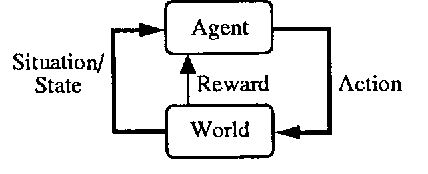
\includegraphics[angle=0,width=0.7\textwidth]{./figs/Dyna-Figure1.png}
		\caption{\label{fig:dyna}The Problem Formulation Used in Dyna. The agent's objective is to maximize the total reward it receives over time. \citep{Dyna}}
	\end{figure}
	\section{Reinforcement Learning}
%	\label{sec:rl}
%	see Fig.~\ref{fig:image}	

	\subsection{Markov Decision Problem}
	A Markov Decision Problem (MDP) is a model for problems, where an agent tries to interact with the environment in such way that the utmost reward is achieved. Specifically, the robot is moving (\textit{transition}) through various \textit{states}, having chosen a specific \textit{action} in each state. Each \textit{reward} is determined by initial state, the action and the following state. 
	All transitions are not deterministic, but rather probabilistic, where each probability only depends on the current state and the current action, see \textbf{Markov Assumption}. That way there has to be one initial state, but multiple end states are possible.\\
	The main goal is to find a reward maximizing \textbf{policiy}, by which the agent selects actions where the maximum reward can be expected.\\
	\begin{itemize}
		\item $S:$ Set of states $\{s_1,s_2,\dots, s_n\}$
		\item $A:$ Set of actions $\{a_1,a_2,\dots, a_n\}$ 
		\item $T: S\times A \times S: $ Transition function, which is the probability of going from state $s$ to state $s'$ via action $a$
		\item $R: S\times A \times S \rightarrow \mathbb{R}: $ Reward function
		\item $\Pi:$ Policy, where an optimal action is assigned to each state
		\item $\gamma \in [0,1]:$ Discount factor. This factor determines the degree of exploration for the agent. For $\gamma=0$, the agent will stick to the policy, and explot the current (possibly) optimal policy. For $\gamma=1$, the agent will take into account the next states reward, leading to exploration behaviour. A value <1 is a contraint, which limits the maximal obtainable reward, leading to a reduction of cycles.
	\end{itemize}
	The \textbf{V-Values} and \textbf{Q-Values} are certain grading schemes used to solve MDPs. It is the total reward the agent can expect, if it performs the optimal, or maximally benefitting, action $a$ in state $s$, and continues to act optimally.
	\begin{equation}\label{eq:vvalue}
		V^*(s) = \max_{a \in A} \sum_{s' \in S}^{} T(s,a,s')[R(s,a,s')+\gamma V^*(s')]
	\end{equation}
	As the values from equation \ref{eq:vvalue} is hard do compute, a technique called \textbf{Value Iteration} is used. It is used do discretize the equation: 
	\begin{equation}\label{eq:value-iteration}
		V^*(s) = \max_{a \in A} \sum_{s' \in S}^{} T(s,a,s')[R(s,a,s')+\gamma V^*(s')]
	\end{equation}
	where $k$ is the radius from the goal state to the agent. For example, regarding the manhattan norm in a 2D plane, the amount of steps the agent has left until it reaches an end state.\\
	After that, \textbf{Policy Extraction} is performed. It is the assignment of an action to each state, maximizing the expected total reward.
	\begin{equation}
		\Pi^*(s) = \text{arg}\max_{a \in A} \sum_{s' \in S}^{} T(s,a,s')[R(s,a,s')+\gamma V^*(s')]
	\end{equation}
	\begin{itemize}
		\item Einführung \textbf{Markov Decision Problem}
		\item Erklärung der Notation für \textit{state}, \textit{action}, \textit{transition function}, \textit{learning rate}, \textit{discount factor}
		\item Unterschiede \textit{value iteration}, \textit{policy extraction}, \textit{prioritized sweeping}
		\item spätestens hier müsste die Bellman Gleichung stehen:
		
		\item Erklärung Q-Learning, Vorteile, Nachteile
		$$Q(s,a) \leftarrow Q(s,a) + \alpha[r + \gamma \max_{a' \in A}Q(s',a')-Q(s,a)]$$
		\item Exploration/Exploitation TradeOff und Techniken
		\item \textbf{HIER:} Idee des Papers: künstliche Erweiterung des State space umd RL für vergangenheitsabhängige Probleme anwendbar zu machen.
	\end{itemize}
	
	
	\section{GALMO}
	\label{sec:galmo}
	\begin{itemize}
		\item Vorstellung der Ergebnisse des Original Paper (GALMO)
	\end{itemize}
	
	
	\section{Project}
	\label{sec:project}
	\begin{itemize}
		\item Umsetzung von Q-Learning in Python
		\item DQN
		\item Implementierung GALMO?
	\end{itemize}
	
	
	\section{Results}
	\label{sec:results}
	
	
	\begin{figure}[t]
		\centering
		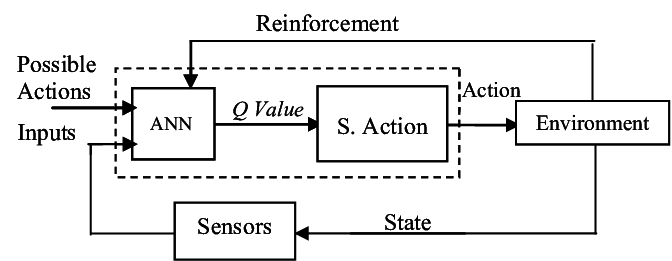
\includegraphics[angle=0,width=0.7\textwidth]{./figs/RL_ANN.png}
		\caption{\label{fig:qlearn}Basic Q-Learning.}
	\end{figure}
	
	
	
	\section{Conclusion}
	
	
	\footnotesize
	\bibliographystyle{plainnat}
	\bibliography{./main}
	
\end{document}
